\section{Empirical Results}
\label{sec:results}

In this section we evaluate our novel SDP solution technique for zero-sum CSGs 
on three continuous domains\footnote{\fontsize{8pt}{10pt}\selectfont All of the source code can be found online at 
\texttt{http://code.google.com/p/xadd-inference}.}: 
(1) continuous stochastic matching pennies; (2) 
binary option stochastic game; and (3) robust energy production. The results represent
the first known exact solutions to these domains. 

\subsection{Continuous Stochastic Matching Pennies}

Matching pennies is a well known zero-sum game with a 
mixed strategy Nash Equilibrium \cite{Osborne_2004}. In this paper we extend 
the standard formulation of the game by incorporating continuous state 
and sequential decisions while still maintaining the zero-sum nature of 
the reward.

\subsubsection{Domain Description}

We define continuous stochastic matching pennies as an extensive
form game between two players $p \in \left\{1, 2 \right\}$. The aim of a 
player is to maximise its expected discounted pay-off at a fixed horizon \emph{H}. 
Our game is played within the interval $[0, 1]$, two fixed variables 
$c \in [0, 1)$ and $d \in (0, 1]$ with $(c < d)$,  are used to partition the interval into
three regions $r \in \left\{1, 2, 3 \right\}$. Each region is associated 
with its own zero-sum reward structure. The continuous state variable 
$x \in [0, 1]$ is used to specify which region the players are competing within.

At each horizon $(h \leq H)$ each player executes an action $a_p \in \left\{ heads_p, tails_p \right\}$. 
Player 1 ``wins'' if both players choose the same action. Otherwise, Player 2 wins. 
The joint actions of the players affect the state $x$ as follows:

{\small 
\abovedisplayskip=0pt
\belowdisplayskip=0pt
\begin{align*}
&P(x' | x, a_{1}, a_{2}) = \\
& \hspace{10pt} \delta \left[ x' - \begin{cases}
      (heads_{1}) \wedge (heads_{2}) \wedge (x \geq k) : & x - k \\
      (heads_{1}) \wedge (tails_{2}) \wedge (x \leq 1) : & x + k \\
      (tails_{1}) \wedge (heads_{2}) \wedge (x \geq k): & x + k \\
      (tails_{1}) \wedge (tails_{2}) \wedge (x \leq 1) : & x - k  \\
    \end{cases} \right]
\end{align*}
}%

The constant $k \in (0, 1)$ is a step size which perturbs the state $x$. 
If Player 1 wins, the state moves to the left by $k$, otherwise it moves to the
right by $k$. The Dirac function $\delta[\cdot]$ ensures that the transitions are valid 
conditional probability functions that integrate to 1. 

We define the rewards obtained by Player 1 in region $r$ as:

{\small 
\abovedisplayskip=0pt
\belowdisplayskip=0pt
\begin{align*}
\label{eq:cmpreward}
  R^r_{1} &= 
    \begin{cases}
     (heads_{1}) \wedge (heads_{2}) : & \alpha^{r}_{1} \\
     (heads_{1}) \wedge (tails_{2}) : & \alpha^{r}_{2} \\
     (tails_{1}) \wedge (heads_{2}) : & \alpha^{r}_{3} \\
     (tails_{1}) \wedge (tails_{2}) : & \alpha^{r}_{4} \\
    \end{cases}
\end{align*}
}%

Here we restrict $\alpha^{r}_i \in \mathbb{R}$. The rewards obtained 
by Player 2 in the same region are simply $-R^r_{1} $. Given this reward 
formulation we specify two different reward structures:
symmetric and asymmetric. In a symmetric reward structure $\alpha^{r}_1 = \alpha^{r}_4$ 
and $\alpha^{r}_2 = \alpha^{r}_3$. An example of this reward structure 
is shown in Table~\ref{tab:smpsymreward}. Under a symmetric reward
setting the expected reward for each player is the same across all regions \textit{r}. 
In an asymmetric reward structure we allow each of the
$\alpha^{r}_i$ to differ in both sign and magnitude. Table~\ref{tab:smpasymreward}
shows an example of an asymmetric reward structure. Under an asymmetric
setting the expected reward for each player may vary across each region \textit{r}. This gives
a player an incentive to reach regions with a higher expected reward.

\begin{table}[h!]\small
\caption{Symmetric reward structure for Player 1.}
\label{tab:smpsymreward}
\begin{tabular}{ l | c | c | c |}
\cline{2-4}   
  & Region 1 & Region 2 & Region 3 \\ \hline
  \multicolumn{1}{ |l| }{$(heads_{1}) \wedge (heads_{2})$}  & 10 & 5 & 20 \\ \hline
  \multicolumn{1}{ |l| }{$(heads_{1}) \wedge (tails_{2})$}     & -10 & -5 & -20 \\ \hline
  \multicolumn{1}{ |l| }{$(tails_{1}) \wedge (heads_{2})$}     & -10 & -5 & -20 \\ \hline
  \multicolumn{1}{ |l| }{$(tails_{1}) \wedge (tails_{2})$}        & 10 & 5 & 20 \\  
  \hline
\end{tabular}
\end{table}

\begin{table}[h!]\small
\caption{Asymmetric reward structure for Player 1.}
\label{tab:smpasymreward}
\begin{tabular}{ l | c | c | c |}
\cline{2-4}   
  & Region 1 & Region 2 & Region 3 \\ \hline
  \multicolumn{1}{ |l| }{$(heads_{1}) \wedge (heads_{2})$} & 1 & 5 & 7 \\ \hline
  \multicolumn{1}{ |l| }{$(heads_{1}) \wedge (tails_{2})$} & -3 & -5 & -2 \\ \hline
  \multicolumn{1}{ |l| }{$(tails_{1}) \wedge (heads_{2})$} & 0 & -5 & 10 \\ \hline
  \multicolumn{1}{ |l| }{$(tails_{1}) \wedge (tails_{2})$} & 2 & 5 & 20 \\  
  \hline
\end{tabular}
\end{table}

\subsubsection{Results}

We investigate the continuous stochastic matching pennies game under
both symmetric and asymmetric rewared structures. For both experiments
the threshold values are set to $c = 0.3$ and $d = 0.7$. The step size is $k = 0.3$.

%------------------------------------------------------------------------------
% Figure
\begin{figure}[]

\begin{subfigure}[b]{0.5\textwidth}
\centering
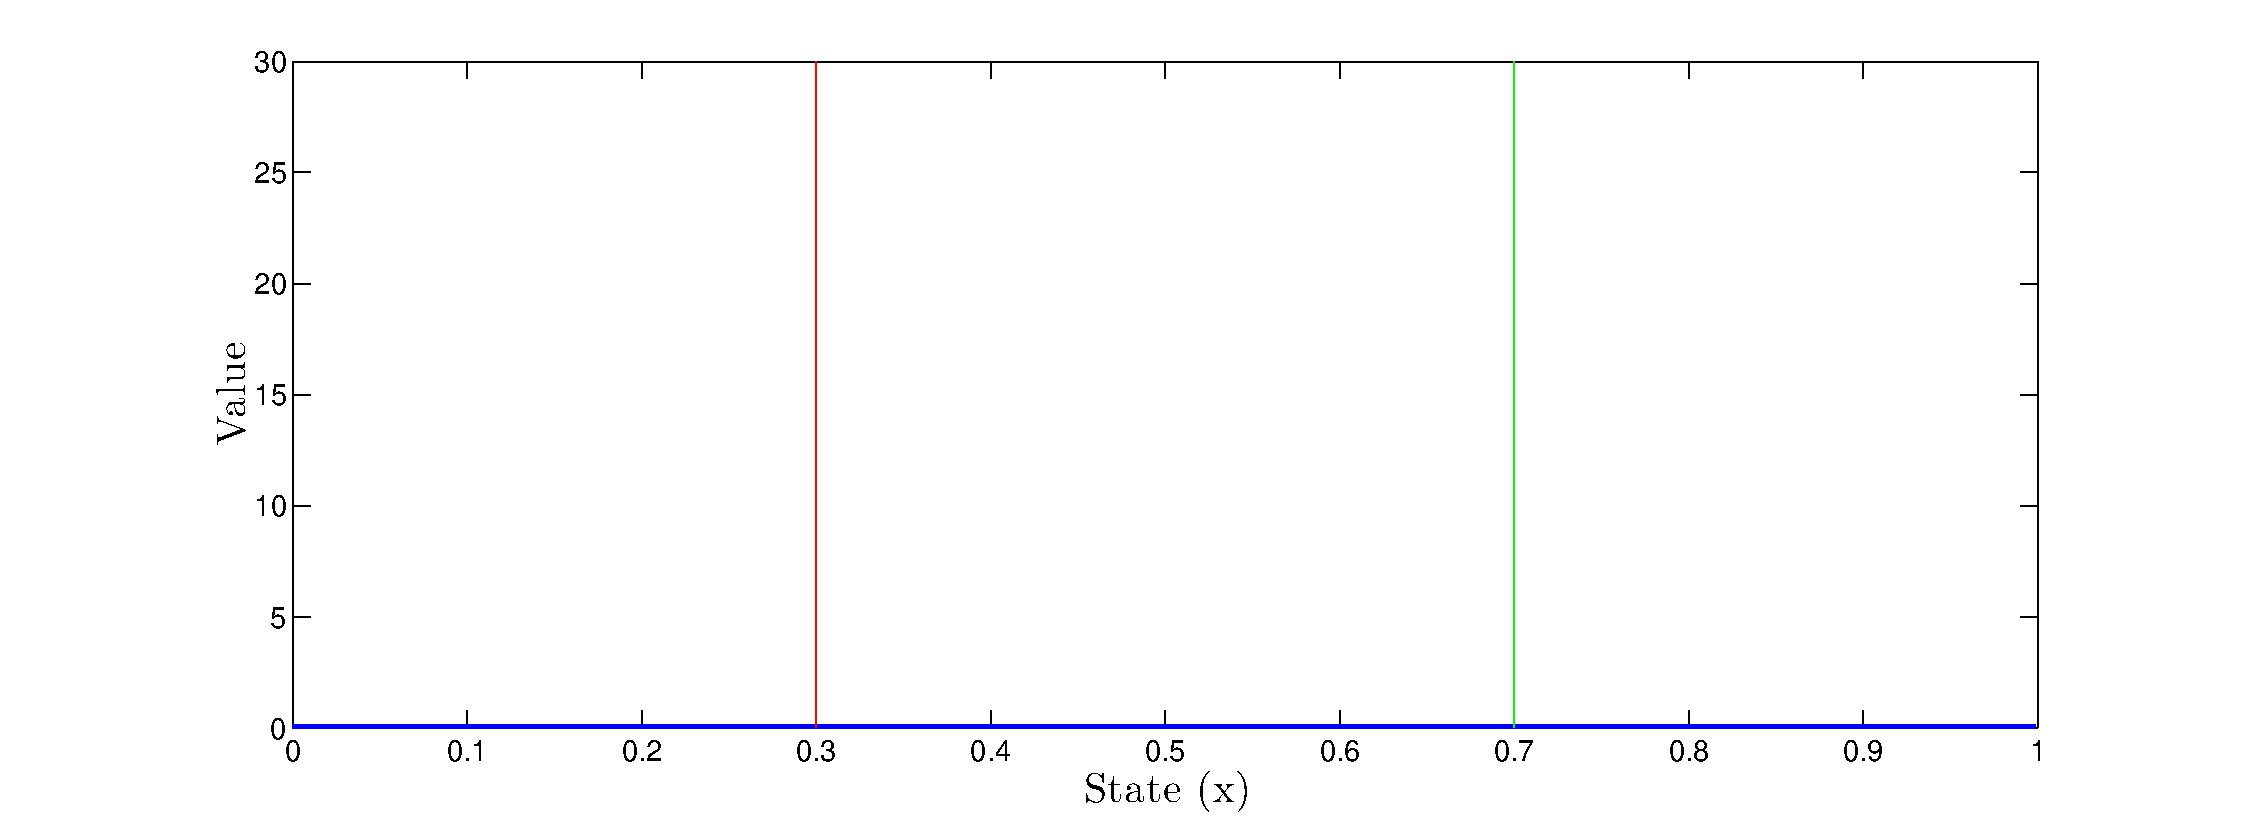
\includegraphics[width=260pt]{smp_sym.pdf}
\caption{Symmetric rewards.}
\label{fig:smpasmreward1}
\end{subfigure}

\begin{subfigure}[b]{0.5\textwidth}
\centering
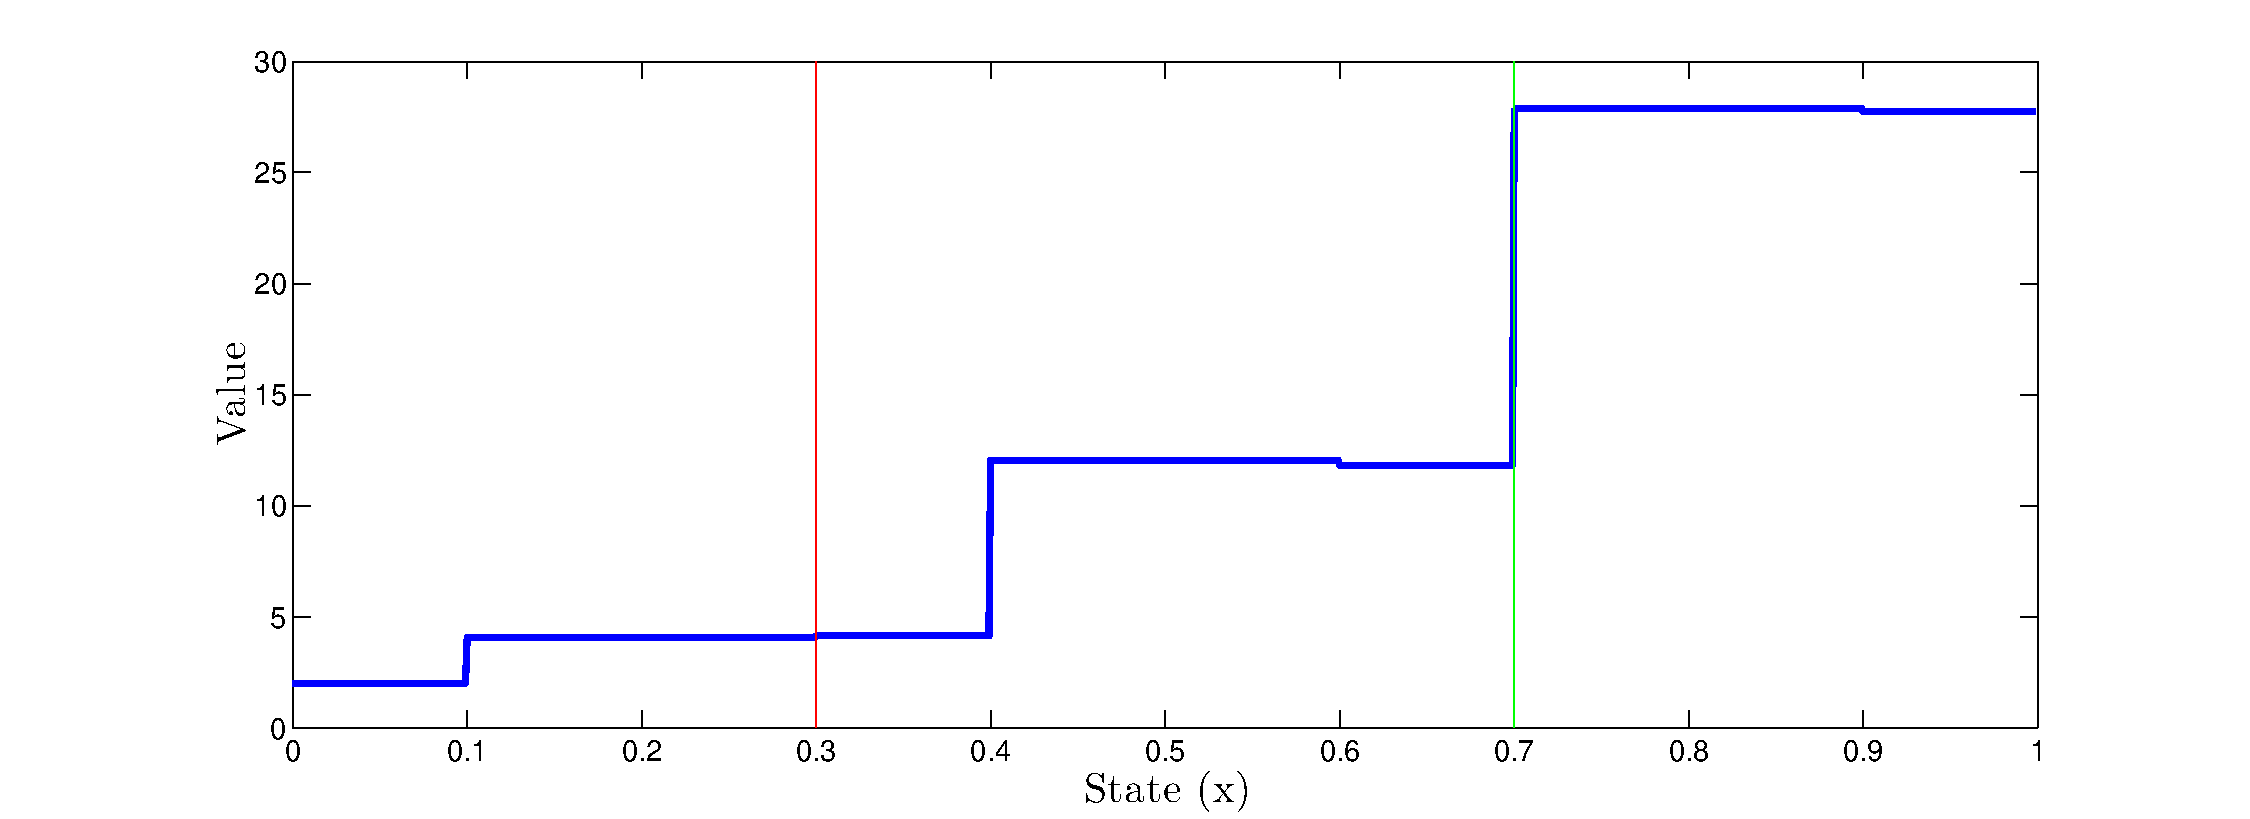
\includegraphics[width=260pt]{smp_asym.pdf}
\caption{Asymmetric rewards.}
\label{fig:smpasmreward2}
\end{subfigure}

%\vspace{-2mm}
\caption{The optimal value functions of the continuous stochastic matching 
            pennies game  for Player 1 at horizon 4 under (a) symmetric and (b) asymmetric reward 
            structures. Threshold values are set to $c = 0.3$
            and $d = 0.7$ and are highlighted in red and green, respectively. 
            The step size is $k = 0.3$.}
\label{fig:smpasmreward}
\end{figure}
%------------------------------------------------------------------------------

Figure~\eqref{fig:smpasmreward1} shows the results of the continuous
stochastic matching pennies game using the symmetric reward structure
given in Table~\ref{tab:smpsymreward}. The results show that the expected 
reward for Player 1 remains at zero over all 4 horizons, irrespective of the state \textit{x}. 
The symmetric reward structure clearly shows that both players achieve
the same expected reward in all regions \textit{r}. This in turn ensures that
both players are indifferent between their pure strategies. Hence, the expected reward 
for each player is zero in all regions. This result corresponds to the well known solution of the 
matching pennies game with symmetric rewards and serves as a proof of concept for 
our novel solution technique.

Figure~\eqref{fig:smpasmreward2} shows the effect of the asymmetric reward structure given in
Table~\ref{tab:smpasymreward}. The figure shows that Player 1 achieves the highest expected
reward in Region 3, followed by Region 2 and finally by Region 1. This corresponds
to the expected reward within each region of Table~\ref{tab:smpasymreward}. The results indicate 
that the Player 1 is no longer indifferent between its pure strategies in each region and may take short-term
losses to reach more favourable regions.

\subsection{Binary Option Stochastic Game}

Binary options are financial instruments which allow an investor to
bet on the outcome of a yes/no proposition. The proposition typically
relates to whether the price of a particular asset that underlies the option
will rise above or fall below a specified amount, known as the strike
price, $\kappa \in \mathbb{R}$. When the option reaches maturity the 
investor receives a fixed pay-off if their bet was correct and nothing otherwise.

\vspace{-1mm}

\subsubsection{Domain Description}

We analyse the valuation of a binary option as an extensive form
zero-sum game between a trader and the market. The aim of the trader
is to maximise their expected discounted pay-off at a fixed horizon $H$ 
through buying and selling options within an adversarial market. 
The problem has two state variables: the underlying market value of the asset
$v \in [0, 100]$ and the trader's inventory of options $i \in \mathbb{N}$.

At each time step the trader can execute one of three actions
$a_{trd} \in \left\{buy_{trd}, sell_{trd}, hold_{trd}\right\}$, where $buy_{trd}$ refers to a request to 
buy an option from the market, $sell_{trd}$ refers to a request to sell an option to
the market and $hold_{trd}$ is equivalent to taking no action. 
The market can execute one of two actions: $a_{mkt} \in \left\{sell_{mkt}, nsell_{mkt} \right\}$,
where $sell_{mkt}$ corresponds to selling an option to the trader and $nsell_{mkt}$ 
corresponds to not selling to the trader. 

The joint actions of the trader and market, $a_{trd}$ and 
$a_{mkt}$, respectively, affect both the underlying market value of the asset
and the trader's inventory. For the sake of simplicity we assume that
the market value may increase or decrease by fixed step sizes, 
$u \in \mathbb{R}$ for an increase and $d \in \mathbb{R}$ for a decrease.

The trader's option inventory dynamics are given by:

{\small 
\abovedisplayskip=0pt
\belowdisplayskip=0pt
\begin{align*}
& P(i' | v, i, a_{trd}, a_{mkt}) = \\
& \hspace{40pt} \delta \left[ i' - \begin{cases}
      (buy_{trd}) \wedge (sell_{mkt}) : & i + 1 \\ 
      (sell_{trd}) \wedge (i > 0) : & i - 1 \\
      otherwise: & i \\
    \end{cases} \right]
\end{align*}
}%

It should be noted that under this formulation the market will always
buy an option from the trader when the trader selects $sell_{trd}$. 
The market value changes according to:

{\small 
\abovedisplayskip=0pt
\belowdisplayskip=0pt
\begin{align*}
& P(v' | v, i, a_{trd}, a_{mkt}) = \\
& \hspace{40pt} \delta \left[ v' - \begin{cases}
      (buy_{trd}) \wedge (sell_{mkt})  : & v + u \\
       (sell_{trd}) \wedge (i > 0) : & v - d \\
      otherwise: & v
    \end{cases} \right]
\end{align*}
}%

Assuming that the strike price $\kappa \in [0, 100]$, the rewards obtained by the trader are given by:

{\small 
\abovedisplayskip=0pt
\belowdisplayskip=0pt
\begin{align*}
  R_{trader} = 
    \begin{cases}
      (sell_{trd}) \wedge (i > 0) \wedge (v > \kappa) : & 1 \\ 
      otherwise : & 0 \\
    \end{cases} \nonumber
\end{align*}
}%

The market's reward is simply the additive inverse of the trader's 
reward. Hence, the binary option game is zero-sum. 

\subsubsection{Results}

%%%%%%%%%%%%%%%%%%%%%%%%%%%%%%%%%
% Figure
\begin{figure}[h!]
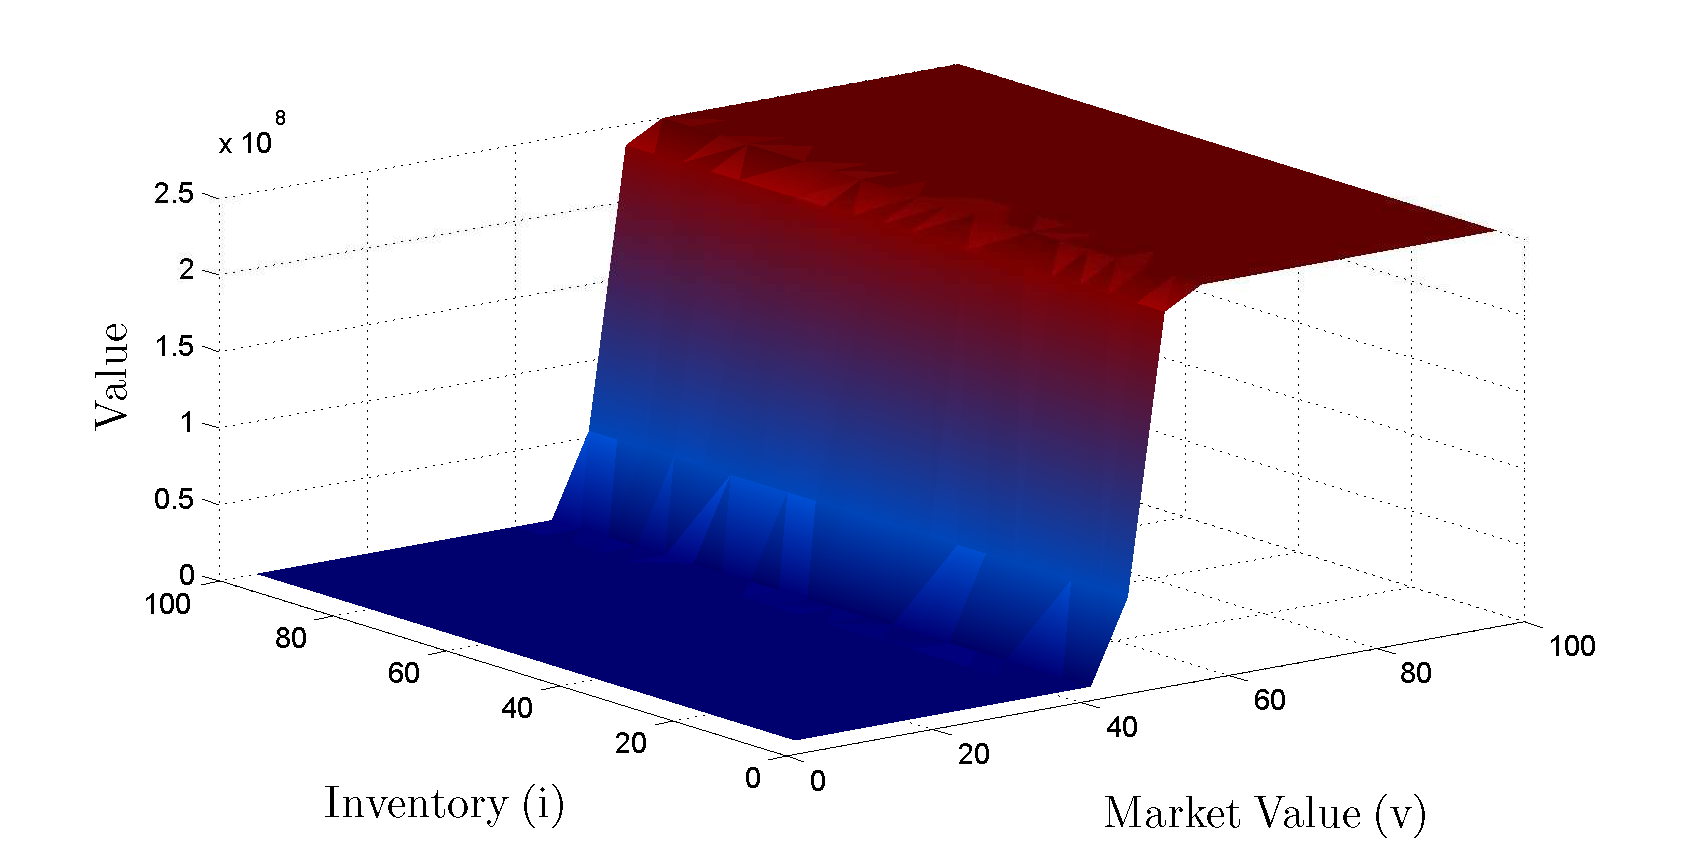
\includegraphics[width=250pt]{sbo.pdf}
%\vspace{-3mm}
\caption{The optimal value function of the binary option stochastic game for the trader at horizon 20. 
The strike price is set to $\kappa = 45.0$ and the increment and
decrement values are set to $u = 1.0$ and $d = 1.0$, respectively. Under the domain specification
the value function is invariant to the inventory $i$. }
\label{fig:binaryoptionvfunc}
\end{figure}
%%%%%%%%%%%%%%%%%%%%%%%%%%%%%%%

In Figure~\eqref{fig:binaryoptionvfunc} we show the optimal value function for the
binary option game at horizon 20. The strike price is set to $\kappa = 45.0$ and
the increment and decrement values, $u$ and $d$ are both set to 1.0. The
value function clearly shows that under this formulation the trader
achieves the most reward by selling options as soon $v > \kappa$.
Selling an option causes the underlying value to decrease. Once the value
falls beneath the strike price, the trader will buy options, which increases
the underlying value. This leads to the continual cycling of buying and selling 
of the option at values close to the strike price $\kappa$. In essence the trader 
behaves like a market maker in that they take both sides of the transaction at values near 
$\kappa$. We note that while Figure~\eqref{fig:binaryoptionvfunc} is invariant to the inventory
of options $i$, its inclusion is critical for the correct formalisation of the domain.

\subsection{Robust Energy Production}

The provision of energy resources is an integral component of any
economy. Energy providers must be able to produce energy in response
to changes in energy demand. In situations where demand exceeds supply,
an energy crisis may occur. In this paper we investigate energy 
production from the viewpoint of an energy provider responsible for 
supplying energy in an adversarial environment.

\subsubsection{Domain Description}

We define our energy production domain as an extensive form zero-sum
game between an energy provider and nature. The aim of the energy
provider is to maximise its expected discounted reward at a 
fixed horizon $H$ by changing production levels in response to changes in demand.
The domain has two state variables: the production level $p \in \mathbb{R}^{+}$ and the energy demand
$d \in \mathbb{R}^{+}$. 

At each time step the energy provider can execute one of two actions
$a_{prd} \in \left\{inc_{prd}, dec_{prd}\right\}$, where $inc_{prd}$ 
refers to increasing energy production and $dec_{prd}$ refers to decreasing
energy production. Nature can also execute one of two actions
$a_{nat} \in \left\{inc_{dem}, dec_{dem}\right\}$, where $inc_{dem}$ 
refers to increasing energy demand and $dec_{dem}$ refers to decreasing
energy demand. We specify the increase in the 
amount of energy produced or demanded by $prd_{u}, nat_{u} \in \mathbb{R}^{+}$ and a
corresponding decrease by $prd_{d}, nat_{d} \in \mathbb{R}^{+}$.

The joint actions of the energy provider and nature, $a_{prd}$ and
$a_{nat}$, respectively, affect the production level as follows:

{\small 
\abovedisplayskip=0pt
\belowdisplayskip=0pt
\begin{align*}
&P(p' | d, p, a_{prd}, a_{nat}) = \\
& \hspace{40pt} \delta \left[ p' - \begin{cases}
      (inc_{prd})  : & p + prd_{u} \\
       (dec_{prd}) \wedge (p > prd_{d}): & p - prd_{d} \\
      otherwise: & p
    \end{cases} \right] & \\    
\end{align*}
}%

The energy demand changes according to:
{\small 
\abovedisplayskip=15pt
\belowdisplayskip=0pt
\begin{align*}
&P(d' | d, p, a_{prd}, a_{nat}) = \\
& \hspace{40pt}\delta \left[ d' - \begin{cases}
      (inc_{dem})  : & d + nat_{u} \\
       (dec_{dem}) \wedge (d > nat_{d}) : & d - nat_{d} \\
      otherwise: & d
    \end{cases} \right] & \\    
\end{align*}
}%

The reward obtained by the energy provider are specified as:

{\small 
\abovedisplayskip=0pt
\belowdisplayskip=0pt
\begin{align*}
  R_{prd} = 
    \begin{cases}
      (p < d) : & -100 \\ 
      otherwise : & 0 \\ 
    \end{cases} \nonumber
\end{align*}
}%

We note that under this reward structure failure to meet energy demand
is heavily penalised, whereas meeting or even exceeding demand are
given the same reward. Nature's reward is simply the additive inverse 
of the energy provider's reward.

\subsubsection{Results}

%%%%%%%%%%%%%%%%%%%%%%%%%%%%%%%%%
% Figure
\begin{figure}[ht!]
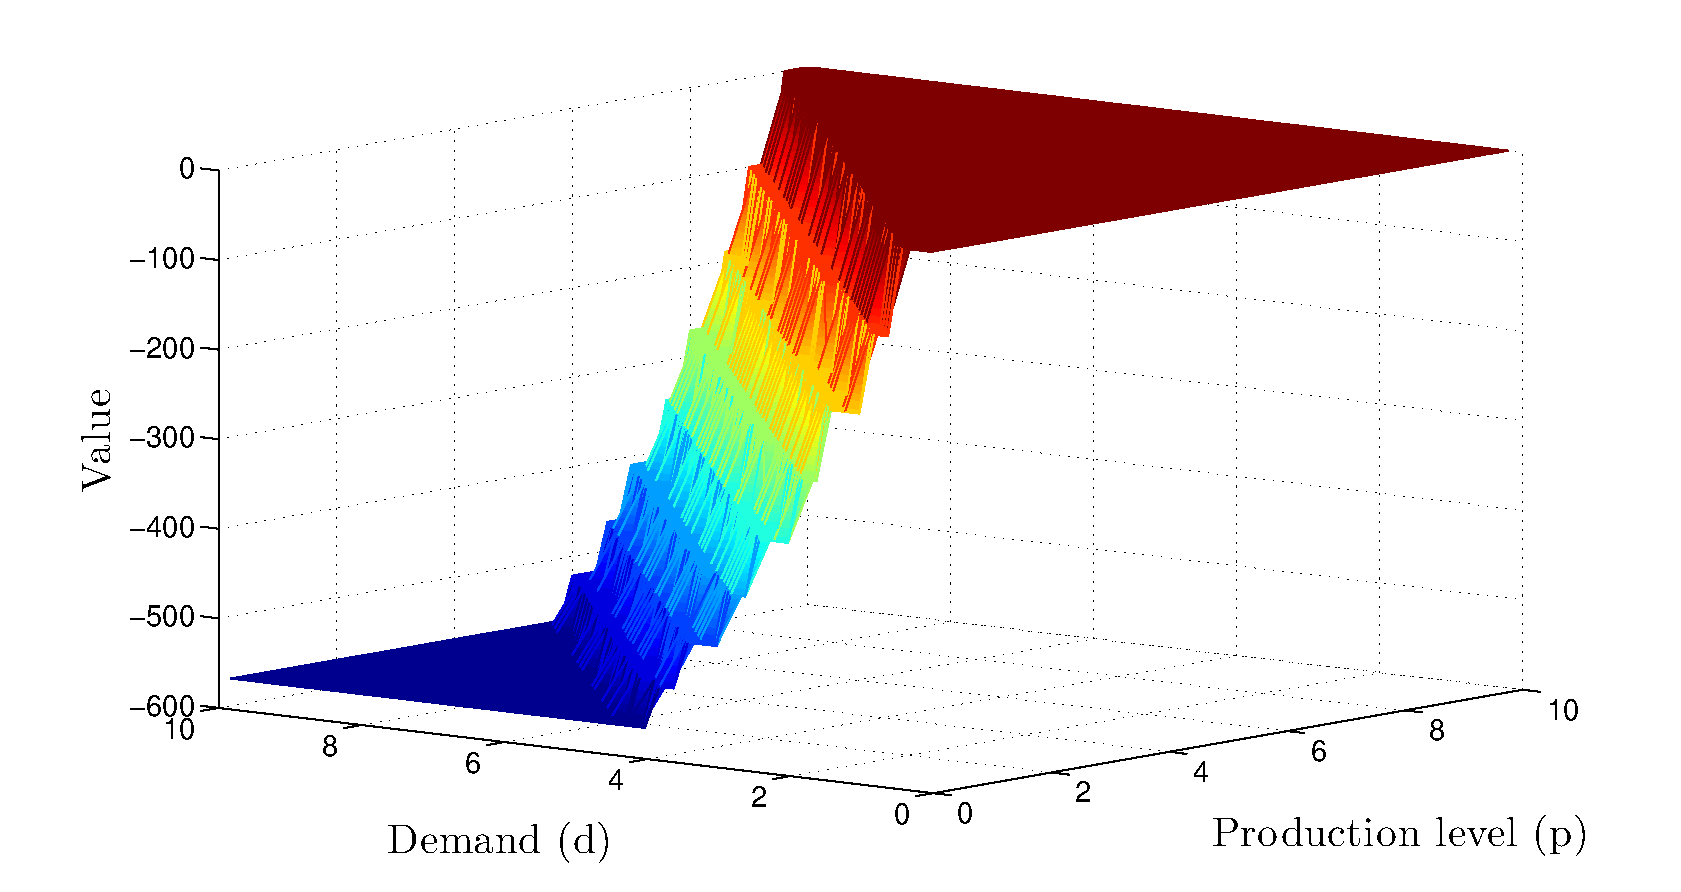
\includegraphics[width=250pt]{sep.pdf}
%\vspace{-3mm}
\caption{The optimal value function of  the robust energy production game for the producer at horizon 8. 
The production and demand increase and decrease variables were set to $prd_{u} = prd_{u} = 1.0$ and 
$nat_{u} = nat_{d} = 0.5$, respectively.}
\label{fig:sepvfunc}
\end{figure}
%%%%%%%%%%%%%%%%%%%%%%%%%%%%%%%%%

In Figure~\eqref{fig:sepvfunc} we show the optimal value function
for the robust energy production game at horizon 8. The production and demand 
increase and decrease variables were set to $prd_{u} = prd_{u} = 1.0$ and $nat_{u} = nat_{d} = 0.5$, respectively.
The value function shows that the energy provider achieves the highest value when the energy provided
meets or exceeds demand. The value function is lowest when the demand exceeds supply, which is in accordance
with the reward structure. The value function clearly decreases in a step-wise manner from the point 
where the production level meets demand, indicating that production levels just beneath demand have a higher value than
those well below demand.
